\documentclass[border=6pt]{standalone}
\usepackage{libertine}
\usepackage[T1]{fontenc}
\usepackage{amssymb}
\usepackage{tikz}
\usetikzlibrary{calc, arrows.meta}
\definecolor{ink}{HTML}{15181C}
\definecolor{accent}{HTML}{C81E5A}
\definecolor{cool}{HTML}{1B6CA8}
\definecolor{figbg}{HTML}{F4F2EE}
\newcommand{\idx}{\phi}
\begin{document}
\begin{tikzpicture}
  % the grey field is a separate layer behind the (transparent) render
  \fill[figbg] (0,0) rectangle (17cm,6.7952cm);
  \node[anchor=south west, inner sep=0] (img) at (0,0)
    {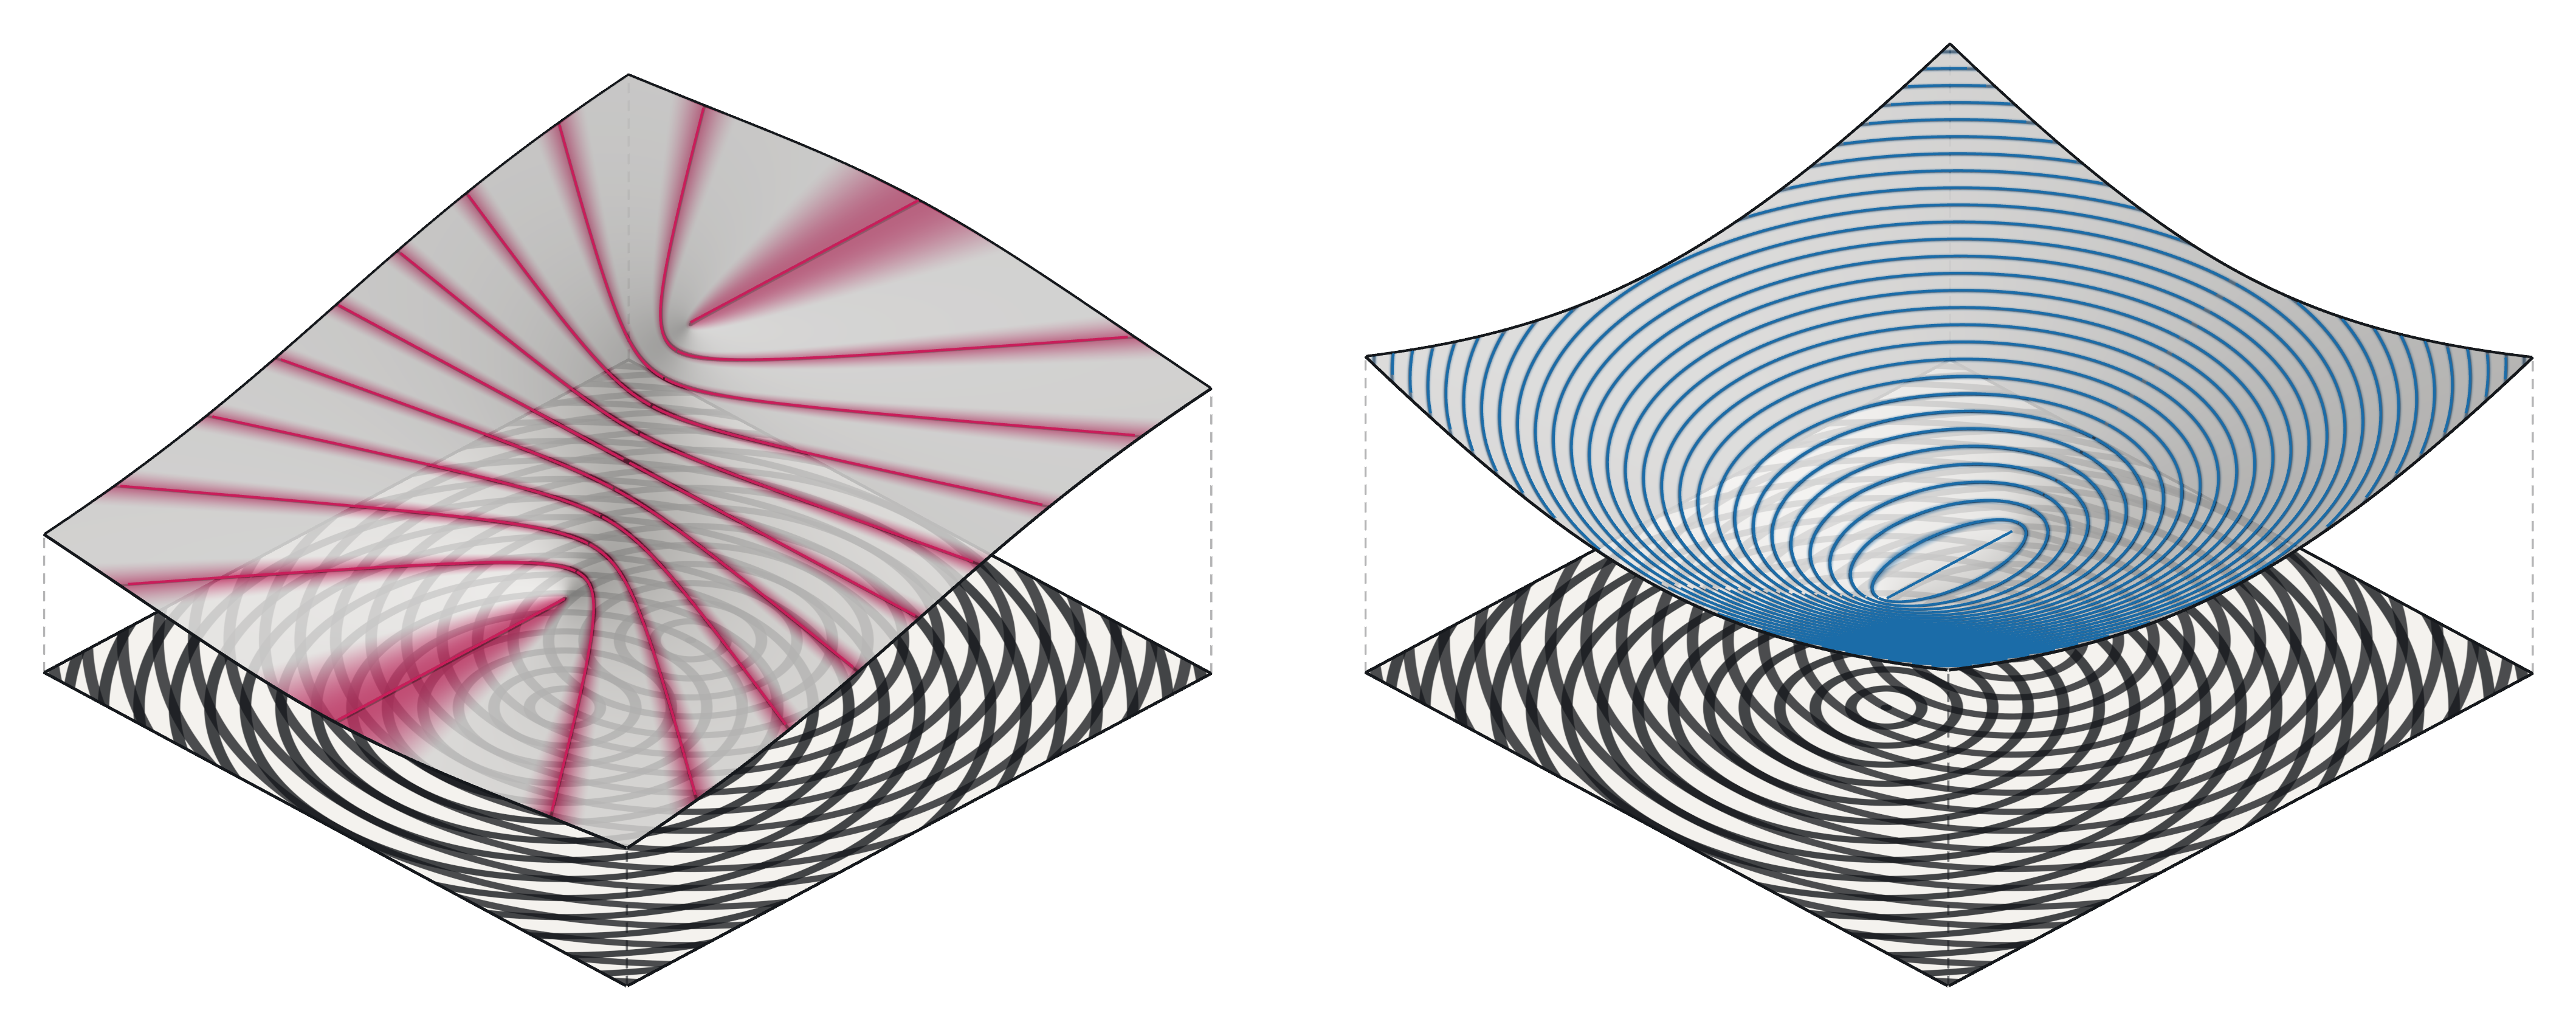
\includegraphics[width=17cm]{fig4-final.png}};
  \begin{scope}[shift={(img.south west)},
      x={($ (img.south east)-(img.south west) $)},
      y={($ (img.north west)-(img.south west) $)}]
    \tikzset{lab/.style={font=\footnotesize, inner sep=1pt}}
    \tikzset{lead/.style={-{Stealth[length=4.5pt]}, line width=0.55pt}}

    % ---------- panel A: the difference ----------
    \node[lab, text=ink, align=left, anchor=west] (gl) at (0.0114,0.8285)
      {the graph of\\$D=\idx_1-\idx_2$};
    \draw[lead, ink!65] (gl.south) to[out=-69,in=132] (0.0905,0.607);

    \node[lab, text=accent!88!ink, anchor=west] (cl) at (0.3873,0.8567)
      {contours at $D\in\mathbb{Z}$};
    \draw[lead, accent!75] (cl.south) to[out=-155,in=90] (0.4113,0.6706);

    \node[lab, text=ink!70, anchor=west] (rl) at (0.0586,0.0309)
      {two ring families};
    \draw[lead, ink!55] (rl.east) to[out=10,in=205] (0.278,0.110);

    % ---------- panel B: the sum ----------
    \node[lab, text=cool!90!ink, anchor=east] (sl) at (0.9769,0.8754)
      {the sum $\idx_1+\idx_2$};
    \draw[lead, cool!75] (sl.south) to[out=-109,in=76] (0.8817,0.7531);
  \end{scope}
\end{tikzpicture}
\end{document}
